\lstset{language=C}

\chapter{OpenMP}
\label{chap:openmp}

Writing multi-threaded programs using the raw POSIX threads API is
tedious and error-prone.  It is also not portable, as POSIX threads is
specific to Unix systems.  Also, writing efficient multi-threaded code
is difficult, as thread creation is relatively expensive, so we should
ideally write our programs to have a fixed number of \emph{worker
  threads} that are kept running in the background, and periodically
assigned work by a scheduler.  In many cases, particularly within
scientific computing, we do not need the flexibility and low-level
control of POSIX threads.  We mostly wish to parallelise loops with
iterations that are \emph{independent}, meaning that they can be
executed in any order without changing the result.  For such programs
we can use \emph{OpenMP}.  We will use only a small subset of OpenMP
in this course.

\section{Basic use of OpenMP}

OpenMP is an extension to the C programming language\footnote{OpenMP
  is not C specific, and is also in wide use for Fortran.} that allows
the programmer to insert high-level \emph{directives} that indicate
when and how loops should be executed in parallel.  The compiler and
runtime system then takes care of low-level thread management.  OpenMP
uses the the \emph{fork-join} model of parallel execution: a program
starts with a single thread, the \emph{master thread}, which runs
sequentially until the first \emph{parallel region} (such as a
parallel loop) is encountered.  At this point, the master thread
creates a group of threads (``fork''\footnote{Note an unfortunate
  mix-up of nomenclature: this has nothing to do with the Unix notion
  of \texttt{fork()}, which creates \emph{processes}, not
  \emph{threads}}), which execute the loop.  The master thread waits
for all of them to finish (``join''), and then continues on
sequentially.  This is called an \textit{implicit barrier}: a point
where execution pauses until all threads reach it.  For example:

\begin{lstlisting}[mathescape=true]
#pragma omp parallel for
for (int i=0; i<n; i++) {
  A[i] = A[i]*2;
}
\end{lstlisting}

The \lstinline{#pragma omp parallel for} line is an OpenMP directive
that indicates that the iterations of the following \texttt{for} loop
can be executed in parallel.  If this loop is compiled with a compiler
that supports OpenMP, the \texttt{n} iterations of the loop will be
divided among some worker threads, which will then execute them in
parallel.

The number of threads used can be controlled at run-time, and is
usually not equal to the number of iterations in the parallel loop.
This is because when the amount of work per iteration is small (as
above), it would not be efficient to have one thread per iteration.

One important idea behind OpenMP is that to understand the semantics
of a program, we can always remove the directives and consider what
the remaining sequential C program would compute.  This is called the
\emph{sequential elision}.  This is a great advantage over low-level
multi-threaded programming.

When we ask OpenMP to parallelise a loop, we solemnly swear that the
following \lstinline{for} loop is actually parallel.  If we break this
vow then the parallel and sequential execution of the code will give
different results; the API does not provide any guarantees about the
absence of race-conditions.  For example, the iterations of the
following loop are not independent, yet OpenMP will not stop us from
asking it to be executed in parallel:

\begin{lstlisting}[mathescape=true]
sum = 0;
#pragma omp parallel for
for (int i=0; i<N; i++) {
  sum += A[i];
}
\end{lstlisting}

Since all threads executing the parallel region have access to the
same data, it is easy to have accidental race conditions in OpenMP
programs.  In \cref{chap:dependencies} we will look in detail at
determining when it is safe to execute a loop in parallel, and how to
transform loops so they become safe to execute in parallel.

\subsection{Compiling and running OpenMP programs}

To compile with support for OpenMP directives in \texttt{gcc}, pass
the \texttt{-fopenmp} option to the compiler. The number of threads
that are going to be used for parallel execution can be set by
environment variable \texttt{OMP\_NUM\_THREADS}.  For example,

\begin{verbatim}
$ export OMP_NUM_THREADS=8
\end{verbatim}

sets the environment variable for the current shell session, such that
any OpenMP we run will use eight threads.  Determining the optimal
number of threads to use for a given program on a particular machine
is something of a black art.  In practice, we just try a few different
numbers and see what runs fastest.

\begin{figure}
\lstinputlisting[
caption={A very simple example of using OpenMP.},
label={lst:openmp-example},
language=C,
frame=single]
{src/openmp-example.c}
\end{figure}

For example, suppose the contrived program in
\cref{lst:openmp-example} is stored in the file
\texttt{openmp-example.c}.  We can then compile as follows:

\begin{verbatim}
$ gcc -o openmp-example openmp-example.c -fopenmp
\end{verbatim}

And then run with various values of \lstinline{OMP_NUM_THREADS} to
investigate the impact of parallelisation:

\begin{verbatim}
$ time OMP_NUM_THREADS=1  ./openmp-example
real    0m0.124s
user    0m0.034s
sys     0m0.090s
$ time OMP_NUM_THREADS=2  ./openmp-example
real    0m0.076s
user    0m0.033s
sys     0m0.104s
$ time OMP_NUM_THREADS=4  ./openmp-example
real    0m0.054s
user    0m0.039s
sys     0m0.133s
$ time OMP_NUM_THREADS=8  ./openmp-example
real    0m0.046s
user    0m0.054s
sys     0m0.184s
\end{verbatim}

Note how the \emph{real} time drops as we use more threads---although
it's not quite eight times as fast with eight threads as with one.
This is likely because this contrived program does so little work
compared to the amount of memory we are accessing.

\subsection{Parallelism versus Concurrency}

The terms \emph{parallelism} and \emph{concurrency} are frequently and
historically used interchangeably.  If you look then up in a
dictionary, you will find them to have almost the same definitions.
In computer science, they are terms of art with distinct (although
related) meanings.

To illustrate concurrency, consider a video game, which from a
programming perspective is basically a real-time interactive
simulation.  Many things need to happen concurrently:

\begin{itemize}
\item We need to figure out what sounds and music to play and send it
  to the IO device connected to the speakers.
\item Many times per second, we need to draw to the screen a rendering
  of the world as observed by the player.
\item Perhaps we wish to guess at where the player is headed next, and
  preload those parts of the game world.
\item We need to run artificial intelligence for computer-controlled
  enemies.
\item We need to compute physics interactions.
\item In a multiplayer game, we need to transmit information
  information about the local game world to other players across the
  network, as well as incorporate information we receive in return.
\item Probably we also wish to perform cleanup tasks, such as removing
  objects from the game world that after a while are no longer
  necessary (e.g. the remains of deceased enemies), to clear up system
  resources.
\end{itemize}

From a programming perspective, it is nicer if we can write each of
these parts as separate flows of control. The artificial intelligence
code should not worry about constantly checking whether it's time to
draw a new screen frame, or whether the player hit some key.
Similarly, the rate at which we receive information from the network
is completely unpredictable, relative to our other responsibilities.

One solution is to implement each of these parts as a distinct thread,
and depend on the operating system to \emph{context-switch} between
them as needed. Maybe we can also use some form of \emph{scheduling
  policy} that understands that it's more important for the threads
responsible for music and graphics to run when they need to, than the
thread that cleans up dead objects or simulates physics. If we have
only a single processor, then all these different threads run
\emph{concurrently}, in that they overlap in time, but only one will
physically be executing instructions at any given point in time. This
means that concurrency can be a useful programming model even when the
goal is not to make the program faster. For that matter, threads are
not the only way to implement concurrency---asynchronous event loops
are a popular technique for highly scalable web servers, but outside
the scope of this course.

\begin{definition}[Concurrency]
  Concurrency is the use of multiple, possibly interacting, logical
  flows of control.
\end{definition}

\emph{Parallelism} is about making programs faster by performing
several computations at the same time.  When we have a program with
multiple threads, such as the video game example above, then if we
have a machine with more than one processing core (which is
essentially every machine these days), we can run several of those
threads in parallel.  While in Unix, threads are the fundamental
\emph{implementation mechanism} for obtaining parallelism, we often
program in languages or frameworks that do not directly expose
threads, because they can be difficult to work with.  For example,
OpenMP is a parallel programming model, but for simple parallel loops,
we do not concern ourselves with actual threads, and we only have a
single logical control flow.

\begin{definition}[Parallelism]
  Parallelism is the simultaneous use of multiple processing units,
  with the goal of speeding up a computation.
\end{definition}

In scientific computing we are mostly concerned with parallelising
loops with independent iterations, and not with concurrent flows of
control.  While OpenMP allows us to peek beneath the covers and
interact with the threads that it uses to \textit{implement} the
parallel loop abstraction, there does exist forms of parallelism, and
parallel programming languages, that do not expose this abstraction,
and are truly parallel without exposing any concurrency.

\section{Reductions}

A loop whose iterations are completely independent can be parallelised
with the \lstinline{#pragma omp parallel for} directive, as shown
before.  Another common case is when the iterations are
\emph{almost} independent, but they all update a single accumulator
- for example, when summing the elements of an array.  For such loops,
OpenMP provides \emph{reduction clauses}, as used to compute a dot
product on \cref{lst:openmp-dotprod}.

\begin{figure}
\lstinputlisting[
caption={OpenMP dot product with reduction clause.},
label={lst:openmp-dotprod},
language=C,
frame=single,
lastline=8]
{src/openmp-dotprod.c}
\end{figure}

Note that all iterations of the loop update the same \texttt{sum}
variable.  The reduction clause \texttt{reduction(+:sum)} that we
added to the OpenMP directive indicates that this update is done with
the \lstinline{+} operator.  The compiler will transform this loop
such that each thread gets its own \emph{private} copy of
\texttt{sum}, which they then update independently.  At the end, these
per-thread results are then combined to obtain the final result.

Reduction clauses only immediately work with a small set of built-in
binary operators: \lstinline{+}, \lstinline{*}, \lstinline{-},
\lstinline{&&}, \lstinline{||}, \lstinline{&}, \lstinline{|},
\lstinline{^}, \lstinline{max}, and \lstinline{min}.  It is also
possible to use user-defined functions, but this is beyond the scope
of this text.  The common property shared by these operators is that
they are \emph{associative}, and have a \emph{neutral element}.  By
associativity, we mean that for some operator $\oplus$, we have
\[
  (x \oplus y) \oplus z = x \oplus (y \oplus z).
\]
That is, the ``order of evaluation'' does not matter.  This is what
allows us to partition the iterations of a reduction loop between
multiple threads, without changing the result.  Note that subtraction
and division is \emph{not} associative---this is why OpenMP does not
allow them in a reduction clause.

A neutral element $0_{\oplus}$ for some operator $\oplus$ is a
``natural zero'' that does not change the result of evaluation:
\[
  x \oplus 0_{\oplus} = 0_{\oplus} \oplus x = x
\]
For example, if the operator is addition, then the neutral element is
$0$.  If the operator is multiplication, then the neutral element is
$1$.  OpenMP requires that the initial value of each reduction
variable (\lstinline{sum} for \cref{lst:openmp-dotprod}) is the
neutral element of the operator.

\subsection{Associativity of floating point operations}

Some of you might recall that addition and multiplication of
floating-point numbers is \emph{not} associative, due to roundoff
errors.  Yet we perform a reduction on \lstinline{double} values in
\cref{lst:openmp-dotprod}!  How can that be valid?  The short answer
is that OpenMP allows us to shoot ourselves in the foot if we wish.
In practice, floating-point operations are often \emph{almost}
associative, and we can get useful results by treating them as if they
were.  In particular, there is no reason to believe that a sequential
left-to-right summation of floating-point numbers is going to be more
numerically accurate than a parallelisation of that loop.  This does
mean that an OpenMP program that uses reductions on floating-point
values might compute a different result than the original sequential
program.

\section{Nested loops}
\label{sec:openmp-nesting}

We can prefix every parallelisable \lstinline{for}-loop with an OpenMP
parallelisation directive.  But what happens if we nest multiple
parallel loops such as the following?

\begin{lstlisting}
#pragma omp parallel for
for (int i = 0; i < n; i++) {
#pragma omp parallel for
  for (int j = 0; j < m; j++) {
    ...
  }
}
\end{lstlisting}

In principle, the answer is easy: the original master thread launches
worker threads to handle each of the \texttt{n} outer iterations, and
these individual worker threads may then launch more worker threads to
handle the inner \texttt{m} iterations.  This is called \emph{nested
  parallelism}: iterations of a parallel loop may itself contain more
parallel loops.  The overhead of nested parallelism quickly becomes
significant, in particular if we have recursive functions so that the
nesting is \emph{dynamic}, so in practice it is not widely used in
OpenMP.  In fact, OpenMP implementations are likely to ignore nested
parallelisation directives, unless the \lstinline{OMP_NESTED}
environment variable is set to \lstinline{True} when running the
program.

However, a common case of nested parallelism is iterating across all
elements of a multidimensional array, such as above, where we are
conceptually covering all indexes of an \texttt{n} by \texttt{m}
array.  This is called \emph{regular nested parallelism}, because the
iteration count of the inner loop (\texttt{m}) is \emph{invariant}
(the same) for all iterations of the outer loop.  Such a nested loop
can be collapsed to a single loop that performs \texttt{n*m} iterations:

\begin{minipage}{1.0\linewidth}
\begin{lstlisting}
#pragma omp parallel for
for (int ij = 0; ij < n*m; ij++) {
  int i = ij / m;
  int j = ij % m;
  ...
}
\end{lstlisting}
\end{minipage}

We use division and modulo operations to extract the intended indexes
from the ``combined'' index \texttt{ij}---this is actually the inverse
of the row-major two-dimensional index function.

However, writing code like this is not very nice, as it obscures our
intent.  Fortunately, OpenMP provides the \texttt{collapse} clause
that we can use to tell OpenMP to parallelise multiple \emph{perfectly
  nested} loops.  By perfectly nested, we mean that the outermost
loops contain only a loop, and no other statements.  An example is
shown in \cref{lst:openmp-matadd}, where we tell OpenMP to treat the
two-deep \emph{loop nest} as a single parallel loop.

\begin{figure}[!h]
\lstinputlisting[
caption={Matrix addition with OpenMP.},
label={lst:openmp-matadd},
language=C,
frame=single,
lastline=10]
{src/openmp-matadd.c}
\end{figure}

You should generally use the \texttt{collapse} clause when writing
such perfectly nested loops, which occurs frequently when implementing
matrix operations.  But more generally, it is usually not worth
worrying too much about parallelising all inner loops of an OpenMP
program.  All we have to do is provide enough parallel work such that
all processors on the system have work to do, and as of this writing,
even a very large computer is unlikely to have more than 256 CPU
cores---and on a personal computer, 16 is more likely.

\section{Scheduling}

When we use a directive to ask OpenMP to execute a loop in parallel,
the compiler and runtime system will decide how the iterations should
be distributed among the threads.  By default, OpenMP uses
\emph{static scheduling}.

\begin{definition}[Static scheduling]
  When entering a parallel loop, we assign each thread exactly the
  number of iterations to execute.
\end{definition}

For example, when executing a loop with $n$ iterations on $m$ threads,
we might assign $\frac{n}{m}$ iterations to each thread.

Static scheduling can be non-optimal when a loop is not
\emph{load-balanced}, meaning that not all loop iterations take the
same time.  For such an \emph{imbalanced} loop, some threads may
finish their iterations quickly and then sit idle while the other
threads finish theirs.  In such cases, we can ask OpenMP to use
\emph{dynamic scheduling}.

\begin{definition}[Dynamic scheduling]
  When entering a parallel loop, we assign each thread an iteration.
  When a thread finishes an iteration, it receives a new one to
  execute.
\end{definition}

The advantage of dynamic scheduling is that an idle thread will
receive more work (if any is available).  The disadvantage is that
dynamic scheduling requires additional communication and
synchronisation---while this is done for us by the runtime system, it
carries a performance overhead.

As an example of the benefit of dynamic scheduling, consider
parallelising loops where each iteration computes Fibonacci numbers
using the recursive function defined in \cref{lst:cfib}\footnote{This
  is an inefficient way to compute Fibonacci numbers---we only use as
  an expensive computation that will take some time.}.

\begin{figure}
\lstinputlisting[
caption={Recursive Fibonacci function.},
label={lst:cfib},
language=C,
frame=single,
firstline=4,
lastline=10]
{src/openmp-schedule.c}
\end{figure}

Since computation of $fib(i+1)$ takes over twice the time of $fib(i)$,
we can produce a very imbalanced loop by letting iteration $i$ compute
$fib(i)$.  \Cref{lst:openmp-fib-static} shows how to parallelise this
with a static schedule in OpenMP.  On my machine, for \texttt{n=45},
this program runs in $5.2s$.  We can ask for dynamic scheduling by
using the the \texttt{schedule(dynamic)} clause, as shown on
\cref{lst:openmp-fib-dynamic}.  On my machine, this version runs in
$2.27s$ - a speedup (\cref{sec:speedup}) of $2.29\times$.

\begin{figure}
\lstinputlisting[
caption={Fibonacci loop with static scheduling.},
label={lst:openmp-fib-static},
language=C,
frame=single,
firstline=19,
lastline=22]
{src/openmp-schedule.c}
\end{figure}

\begin{figure}
\lstinputlisting[
caption={Fibonacci loop with dynamic scheduling.},
label={lst:openmp-fib-dynamic},
language=C,
frame=single,
firstline=27,
lastline=30]
{src/openmp-schedule.c}
\end{figure}

By default, dynamic scheduling assigns single loop iterations to
threads.  This is not a problem for the Fibonacci example, because
there are few loop iterations, and they take a fairly long time to
run.  For loops with many iterations, where dynamically scheduling
single iterations at a time would involve too much overhead, we can
add a \emph{chunk size} to the scheduling clause.  For example,
\begin{lstlisting}
#pragma omp parallel for schedule(dynamic, 100)
\end{lstlisting}
will schedule in chunks of 100 iterations at a time.

The \texttt{guided} schedule is similar to \texttt{dynamic}, but
starts out with big chunks and may then decrease the chunk size during
program run-time if the work is imbalanced.

OpenMP's default behaviour will usually do a good job scheduling most
loops.  But if we do not see the performance gains we would expect,
and we see in a process monitor that some of our processors are idle
while our program is running, it is worth considering whether our
loops could benefit from a scheduling clause.

\section{The Big Concurrency Problems}

Concurrency and Parallel programming is a complex task, and can often be 
a study in what not to do. Luckily, OpenMP manages a lot of the underlying system interactions to ensure correct and efficient concurrency, but no system is perfect. If you ever need to debug whats going on, or try to implement your own concurrent solution you will need a firm understanding of the two core problems; race conditions and deadlocks.

\subsection{Races}

\begin{definition}[Race Condition]
  Sometimes also referred to simply as a race. A race condition is any processing whose final result depends on the arbitrary ordering of prior operations.
\end{definition}

Races are a result of concurrent programs least desirable feature, non-determinism. This is due to the essentially random\footnote{Note that in practice the scheduler will not be literally scheduling at random, but that process scheduling is way out of scope for this course. As user of a computer, we also have little to no control over other users and processes that our program may be competing with, so even when we do understand the scheduler it is still treated as effectively random.} scheduling of any threads and processes, so we do not actually know in what order concurrent operations will be performed.

Within threading this is most often caused by global variables being shared among several threads. This is as each thread can read and write to and from the same location, in essentially any order. As an example, consider the code in listing \ref{lst:race-example}. This code will spread the execution of the counting loop across many threads, which will all read, increment and write to count in an arbitrary order. This will produce an output for count that could be any value between 2 up to 1000000. In practice you are \textit{very} unlikely to get a result as low as 2, but it is technically possible if you get the very unluckiest scheduling\footnote{If you're interested in how this is possible you can look through the trace on page 36 of this \href{https://link.springer.com/content/pdf/10.1007/s00165-017-0447-x.pdf}{pdf}}. Of course its just as possible that you get 1000000 but this non-deterministic result is everything we want to avoid in computing. 

\begin{figure}
  \lstinputlisting[
  caption={An example of a racing program.},
  label={lst:race-example},
  language=C,
  frame=single]
  {src/race.c}
\end{figure}
  
\subsection{Locks}

The code in \ref{lst:race-example} will produce a non-deterministic result, which we have already seen how to solve in OpenMP, by adding 'reduction(+:count)' after the 'parallel for' loop. Reductions are great for OpenMP, but a more broadly applicable solution is the use of a mutex. Note that within the wider literature you will see references to mutexes, locks, or semaphores. These are all name for related but slightly different objects but within HPPS, and we will only concern ourselves with mutexes. They are effectively a flag that can only be set by one thread at a time. 

This is achieved via atomic operations. An atomic operation is one that cannot be interrupted. Recall that the problem with race conditions is that we cannot guarantee that a thread will not interrupt another thread, even if it is midway through an operation. Mutexes are implemented at the machine level to only have two operations, set (e.g. claim the mutex) and release (e.g. give up the mutex). Both of these operations are implemented as atomic operations, that the scheduler cannot interrupt. Once a thread has claimed a mutex, then any other threads that try to claim it will be blocked until the mutex is released. This can have the effect of reducing how much parallel processing is taking place, as threads will have to wait for mutexes to be released before they can continue. However, this cost to speed is worth it if it means we can get an actually meaningful result.

\begin{figure}
  \lstinputlisting[
  caption={An example of a mutex fixing a racing program.},
  label={lst:mutex-example},
  language=C,
  frame=single]
  {src/mutex.c}
\end{figure}

An example of how a mutex can be implemented using the 'pthread' library, as is shown in listing \ref{lst:mutex-example}. This example will always produce the correct result, regardless of how many threads are used to calculate it. Note that in this case, the mutex is locking access to the entirety of the parallelised section, meaning that this program will in fact be much slower than the racing program shown in listing \ref{lst:race-example}. We can see this in the timings presented below, when the mutexed version is 3 times slower, as the threads need to keep waiting for each other to release the mutex. This shows us that mutex usage should be minimised, by only locking the smallest number of instructions to ensure we get the correct result. Sometimes a lock is inevitable though, and so if we were going to improve this program we would perhaps restructure the entire code so that each thread calculates a subtotal, and these are then totalled in a mutexed variable. This is in fact what an OpenMP reduction automatically does.

\begin{minipage}{1.0\linewidth}
  \begin{verbatim}
    $ time ./race
    real    0m0.031s
    user    0m0.173s
    sys     0m0.004s
    $ time ./mutex
    real    0m0.102s
    user    0m0.161s
    sys     0m0.484s
  \end{verbatim}
\end{minipage}

\subsection{Deadlock}

Mutexes may help solve the problem of races, but they can introduce a compeletly new problem, deadlock. 

\begin{definition}[Deadlock]
  Any situation where no system progress can take place, as every process/thread is waiting for another to progress before it can.
\end{definition}

Much like races, deadlocks can be non deterministic which can make them twice as annoying to debug, but we must treat the possibility of a deadlock as though it will deadlock eventually. Therefore we need to design our systems so that they are deadlock free. As an example of how a deadlock could occur consider the following two threads, each which just lock and then unlock two mutexes each:


\begin{minipage}{1.0\linewidth}
  \begin{verbatim}
     Thread 1        Thread 2 
      lock(A)         lock(B)
      lock(B)         lock(A)
     unlock(A)       unlock(A)
     unlock(B)       unlock(B)
  \end{verbatim}
\end{minipage}

The ordering of these operations is completely up to the whims of the scheduler. Many orderings of these operations would be fine, but one such bad one would be if thread 1 locked mutex A, but was then immediately interrupted by thread 2 who would then lock mutex B. Thread 2 cannot continue as it cannot lock mutex A, as it is already locked by thread 1. Thread 1 also cannot continue as its next operations is to lock mutex B, but it is locked by thread 2. This is a deadlock, as there is no way for either thread to progress. There is also no way for these two threads to detect that they are in a deadlock, the system is completely stopped with no way to recover.

\subsection{Progress Graphs}

Reasoning about how each thread could be scheduled is all well and good, but a more robust method to identify potential deadlocks would help a lot. We can do so through the use of progress graphs. These are informal sketches, where we can map all the mutex interactions, and can then deduce any potentially deadlocking behaviour. For an example looking to figure \ref{fig:progress-deadlock}. In this type of graph we map each threads progression along the graph axis'. We only need to map any locking and unlocking operations, as anything else may be time consuming but is ultimately a non-blocking operation that will complete in a finite amount of time.

\begin{figure}
  \centering
  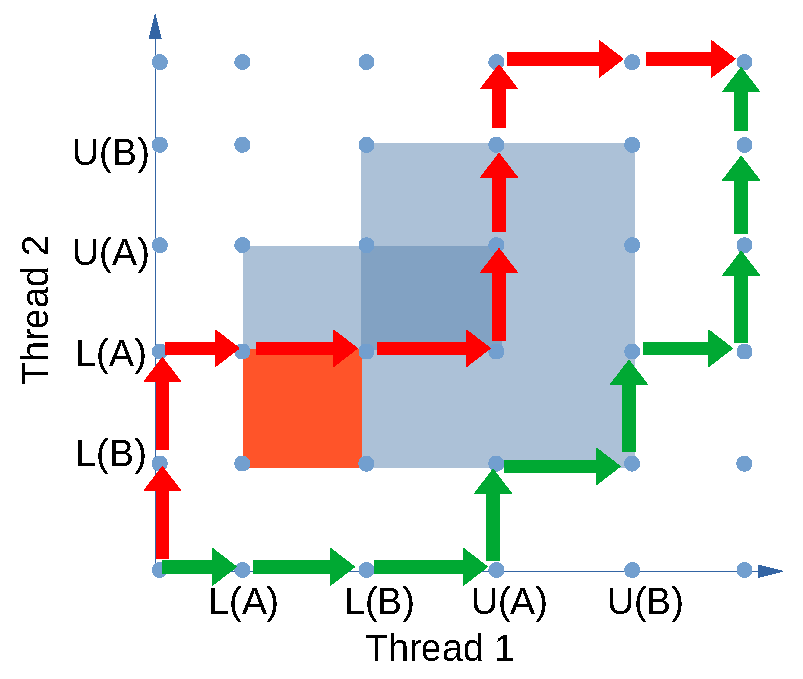
\includegraphics[width=\textwidth]{img/progress-deadlock.pdf}
  \caption{A progress graph of the two potentially deadlocking threads.}
  \label{fig:progress-deadlock}
\end{figure}

As each thread is sequential, its progress can be mapped by following along its axis, with any point in the graph being an expression of the combined states of both graphs. For example, the bottom left corner would be neither thread having started yet, with the top right corner being both threads having completed. The shaded blue section shows forbidden zones, where due to our mutexes is an impossible state to reach. There are two overlapping zones here, one for mutex A and one for mutex B, with them each overlapping in the middle of the graph. We can derive the locations of these zones by taking the coordinate of where each thread locks the mutex as the bottom left corner, and the coordinate of where each thread unlocks the mutex as the top right corner.

Two traces have been shown through the graph, one in green and one in red. The green shows a valid route through that does not enter any forbidden zone and so will produce a valid result. The red is an impossible trace as it enters a state within the forbidden zones, and so cannot occur in practice.

The concerning part of this graph is the red shaded area towards the bottom left of the graph. This shows a potential deadlock. As each thread can only progress linearly, our route through the graph can only be parallel to either axis. If our state ever enters the red zone then there is no way to escape as progress is blocked by the two forbidden zones. This makes it trivial to say that if we can draw a progress graph, if it none of these progress traps exist then our system is deadlock free. A solution to this is to reorder the operations our threads perform. This can be seen in figure \ref{fig:progress-safe} where both threads are now locking and unlocking the mutexes in the same order. No progress traps exist and any valid state has at least one path out of, therefore we are always deadlock free.

\begin{figure}
  \centering
  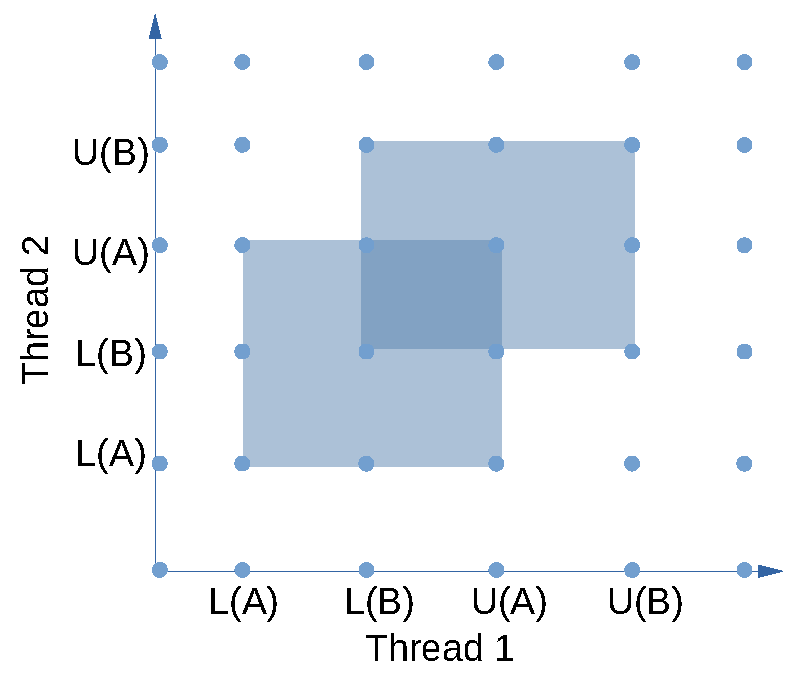
\includegraphics[width=\textwidth]{img/progress-safe.pdf}
  \caption{A progress graph of the two never deadlocking threads.}
  \label{fig:progress-safe}
\end{figure}

%%% Local Variables:
%%% mode: latex
%%% TeX-master: "notes"
%%% End:
